
\documentclass{article}
\usepackage{algorithmicx}
\usepackage{algpseudocode}
\usepackage{algorithm}
\usepackage{graphicx}
\usepackage{amsmath}
\usepackage{subcaption}
\title{Ph.D. Qualifying Examination}
\author{William Curran}
\widowpenalty10000
\clubpenalty10000

\begin{document}

\begin{titlepage}
\maketitle
\tableofcontents
\thispagestyle{empty}
\clearpage
\end{titlepage}

\section{Introduction}
$|S|^{|F|}$
Putting robots into real homes to help those with severe physical disabilities, such as amyotrophic lateral sclerosis (ALS) and quadriplegia, is a long-term goal for our research. Autonomy is one aspect of this goal, however, developing full autonomy for all household tasks for an individual is not possible. We propose to give the user the tools to teach the robot themselves, giving the disabled user both independence and personal customization.

Using a combination of learning from demonstration and reinforcement learning, users can demonstrate to the robot how to perform tasks, and then give feedback via reinforcement learning based on the success of that task. Section 2 and 3 will discuss the current reinforcement learning and learning from demonstration literature, and the tools we can use from each field. 

Human-Robot Interaction analyzes how humans can successfully interact with robots in a social environment. Since our user base are people who suffer from severe physical disabilities, they require specially designed interfaces and tools. Section 4 discusses the current Human-Robot Interaction literature, with an emphasis on assistive robots for those with physical disabilities. Section 5 will look at how to combine learning from demonstration with assitive robots. It will analyze how to develop a learning from demonstration algorithm for people who can't provide a good demonstration physically, and who cannot provide timely or quality feedback to guide the learning. 

\section{Reinforcement Learning}
\label{sec: Reinforcement Learning}
Reinforcement learning is a tool within the field of multiagent or single-agent learning where agents take an action, observe the environment, and receive a reward based on the new environment \cite{Sutton98reinforcementlearning}. Reinforcement learning addresses the problem of finding an optimal policy, $\pi(s,a) = P(a|s)$, that maximizes a reward function, $R$:

\begin{equation}
J(\pi) = \sum_{s,a}\mu^{\pi}(s)\pi(s,a)R(s,a)
\end{equation}
where $\mu^{\pi}(s)$ is the probability distribution over policy $\pi$ (Section \ref{sec:State Transitions}).

To develop this optimal policy, reinforcement learning uses the current state of the agent, $s$, the action taken, $a$, the resultant state, $s'$, and a reward corresponding to the system-level success or failure of the state and action, $R$.

%Reinforcement learners can learn with and without a model of the environment. 

There are three main aspects when defining a stateful reinforcement learner: the policy, the reward function, and the state transitions. 

\subsection{Policy}
The reinforcement learner's policy represents the actions an agent should take in each state. This policy is computed either by a value function representing the quality of a particular action within the state, or a direct search through the policy-space.

\subsubsection{Value Function}

Learning algorithms based on value functions estimate a value function $V^\pi(s)$ that computes the long-term reward of state $s$ to derive a policy $\pi(s)$ \cite{Kalyanakrishnan:2009:EAV:1558109.1558115}. There are two common value function-based methods to estimate $V^\pi(s)$, policy iteration and temporal difference methods.

%Value function based learning algorithms estimate a value function $V^\pi(s)$ that computes the long-term reward of state $s$ to derive a policy $\pi(s)$ \cite{Kalyanakrishnan:2009:EAV:1558109.1558115}. There are two common value function based methods to estimate $V^\pi(s)$, policy iteration and temporal difference methods.
%
%\subsubsection{Policy Iteration}
%Policy iteration and value iteration are a model-based approaches that require the transition probabilities $T(s',a,s)$ (the model) and the reward function $R(s,a)$ to calculate the value function. Policy iteration consists of alternating between policy evaluation and policy improvement. Policy evaluation updates the value function by visiting each state in the current policy, and updating the estimate of $V(s)$ \cite{Braziunas03pomdpsolution}:
%
%\begin{equation} \label{eq:Policy Iteration}
%V_i^\pi(s) \leftarrow R(s,\pi(s)) + \gamma \sum_{s' \in S} T(s,\pi(s),s')V^\pi(s')
%\end{equation}
%
%this update is based on the current value estimates of the successor states $V^\pi(s')$, the state transition probabilities $T(s,\pi(s),s')$, the current policy $\pi$, the reward function $R(s,\pi(s))$ and the discount factor $\gamma$. After the policy is evaluated, the policy is then greedily improved by selecting the best action in every state, according to $V(s)$. Policy evaluation and policy improvement is repeated until the policy has converged.
%
%Value iteration combines the policy evaluation and policy improvement by directly updating $V(s)$ every time the state changed \cite{Braziunas03pomdpsolution}:
%
%\begin{equation} \label{eq:Value Iteration}
%V_i^\pi(s) \leftarrow \max_{a \in A} [R(s,a) + \gamma \sum_{s' \in S} T(s,a,s')V^\pi(s')]
%\end{equation}
%
%Policy iteration and value iteration are both guaranteed to converge to the optimal solution, assuming that we have a model of the environment and infinite time. Both approaches are nearly exhaustive in the search for an optimal policy, and the time complexity includes the size of the state space and action space. In addition, the model of the environment must be completely accurate in order to avoid an accumulation of error. This makes policy iteration difficult to perform in the continuous and large state spaces typically seen in the field of robotics. Current research in reducing the number of states in the system is discussed in Section \ref{sec:Dimensionality}, and methods to compensate for model inaccuracies is discussed in Section \ref{sec:Model Accuracy}. 

Policy iteration and value iteration are model-based approaches that require the transition probabilities $T(s',a,s)$ (the model) and the reward function $R(s,a)$ to calculate the value function. Policy iteration consists of alternating between policy evaluation and policy improvement. Policy evaluation updates the value function by visiting each state in the current policy, and updating the estimate of $V(s)$ \cite{Braziunas03pomdpsolution}. Policy improvement then picks the policy considered optimal. Learning stops when policy improvement converges.

Policy iteration and value iteration guarantee convergence to the optimal solution, assuming that we have a model of the environment and infinite time \cite{Russell:2009:AIM:1671238}. Both approaches are nearly exhaustive in the search for an optimal policy, and the time complexity includes the size of the state space and action space. In addition, the model of the environment must be completely accurate in order to avoid accumulation of error. This makes policy iteration difficult to perform in the continuous and large state spaces typically seen in the field of robotics.

Alternatively, temporal difference methods use the reward received at each time step to calculate the difference between the old estimation of the value function and the new estimation. One such example is Q-Learning \cite{Sutton98reinforcementlearning}.

%\begin{equation}
%Q_{t+1}(s_t,a_t) \leftarrow Q_t(s_t,a_t) + \alpha [R_{t+1}(s_t,a_t) + \gamma \max_a Q_t(s_{t+1},a) - Q_t(s_t,a_t)]
%\end{equation}

%where $R_{t+1}(s_t,a_t)$ is the reward after taking action $a_t$ in state $s_t$, $\alpha$ is the learning rate, and $\gamma$ is the discount factor weighting the value of future rewards.

In contrast to policy iteration approaches, the temporal difference learner does not perform a search of all successor states. The agent is required to arbitrarily explore previously unseen states or unused actions. In order to find an optimal policy, the agent visits as much of the state-action space as possible. This can result in large and sudden modifications to the current policy. This instability is not desired in robotics, since the robot can be easily damaged. Cautious exploration must be enforced by either avoiding significant changes in the policy (enforcing stability) \cite{Peters+MA:2010}, or strictly disallowing the entering of undesired states \cite{conf/rss/DeisenrothRF11}.

Temporal difference methods also guarantee convergence to the optimal solution, with the same assumptions of infinite time \cite{Russell:2009:AIM:1671238}. Since these methods do not require the search of all successor states, the computational complexity is much lower. Temporal difference learning methods are the most widely used methods in reinforcement learning due to the simplicity, minimal amount of computation, and fewer constraints than alternative methods \cite{Sutton98reinforcementlearning}.

Value function approaches are compact, simple, and have been proven to find an optimal policy \cite{raey}. However, in order to obtain these optimality guarantees, nearly the complete state-action space must be visited, which is often computationally intractable in robotics. In addition, the value function must be discretized when used in a continuous state or action space problem, which can lead to approximation errors. Approximation errors can lead to errors in the value function, which can propagate throughout the policy \cite{journals/ftrob/DeisenrothNP13}.

%TODO: Talk about exploration.
\subsubsection{Policy Search}

Policy search algorithms are the reinforcement learning approach of choice in robotics \cite{journals/ftrob/DeisenrothNP13, raey}. Policy search methods use parameterized policies, rather than a value function, essentially performing local explorations through policy space. %The general goal of policy search is to optimize the policy parameters $w$ such that the expected return:

%\begin{equation}
%J(w) = E [\sum \alpha r_k]
%\end{equation}
%is optimized, where $\alpha$ is the discount factor.

Parameterized policies enable reinforcement learning to scale to high dimensional and continuous action spaces by reducing the space of possible policies. Although the localized policy search removes the convenient optimality guarantees of value function reinforcement learning, it includes the benefits of better scalability \cite{journals/ftrob/DeisenrothNP13, raey}, more intuitive policy initialization with expert knowledge \cite{4058714}, and stability \cite{Bertsekas:2000:DPO:517430}. 

Given that policy $\pi$ is parameterized by the set of parameters $w$, the most general policy representation is: 

\begin{equation}
\pi(s) = w^T \theta(s)
\end{equation}
where $\theta(s)$ is a basis function vector, typically linear in simple problems, and nonlinear with additional free parameters in more complex problems. Alternatively, policies can be represented by a function approximation, such as a neural network \cite{Heidrich-Meisner:2009:NSE:1645448.1645634}. 

Similar to value function approaches, policy search repeats a three step process: exploration of the state space, evaluation of the policy, and the update of the current policy. The exploration strategy is an important step in policy improvement for all reinforcement learning approaches and was discussed in the previous section.  

There are two types of policy evaluation when performing policy search, step-based and episodic. The step-based policy evaluation is identical to the iterative policy evaluation approach used in value function learning. The quality of an action is given by the expected future reward of executing an action in a specific state. Value function approaches can be used in this case, as well as a Monte-Carlo estimation. %Many well established policy search algorithms, such as PoWER \cite{Kober:2011:PSM:2004157.2004158}, PI$^2$ \cite{Theodorou:2010:GPI:1756006.1953033}, and REINFORCE \cite{Williams92simplestatistical}, employ the step-based technique.

The episodic policy evaluation uses the expected return of the entire learning episode to update the parameter vector $w$. Rather than updating the value function associated with a specific state-action pair, episodic policy evaluation evaluates the policy parameters directly. %Policy search algorithms have used episode-based evaluations with success, such as Episode-Based PI$^2$ \cite{DBLP:journals/corr/abs-1206-4621}, Parameter Exploring Policy Gradient (PEPG) \cite{conf/icann/SehnkeORGPS08}, and CMA-ES \cite{Hansen:2003:RTC:772374.772376}.

Once a policy is evaluated, it needs to be updated based on the resultant evaluation of the state-action pair or the policy parameters. Most policy search research focuses on improving the policy update step with respect to maximizing sample efficiency, minimizing the number of tunable parameters, and increasing learning stability \cite{journals/ftrob/DeisenrothNP13}. There are many mathematical approaches for policy update, including policy gradient \cite{Baxter99directgradient-based, kohl:icra04, 4058714, Shu:2006:NCL:1666642.1666764,Williams92simplestatistical}, expectation-maximization \cite{Kober:2011:PSM:2004157.2004158, conf/icml/Neumann11}, and information-theoretic approaches \cite{DanielAISTATS2012, Peters+MA:2010}.

Policy gradient approaches are direct, in that they directly compute the gradient to maximize policy performance. The REINFORCE algorithm was one of the first policy search algorithms, performs well, and computes policy updates without explicitly computing gradient estimates \cite{Williams92simplestatistical}. However, these approaches require the user to specify a learning rate, which can lead to instability or slow learning if not chosen correctly.

Expectation-Maximization methods remove the need for a learning rate. Variational Inference for Policy Search (VIP) is a typical example. It uses inference to autonomously determine the exploration rate and learning rate \cite{conf/icml/Neumann11} but these approaches can potentially have an unstable learning process as well as tends to converge to local minima \cite{journals/ftrob/DeisenrothNP13}. 

Information-theoretic approaches are considered the best for policy search, as they combine the benefits from both policy gradient and expectation-maximization approaches \cite{journals/ftrob/DeisenrothNP13}. Information-theoretic approaches bound the distance between the prior policy and the new policy at each update step, enforcing stability in the learning process, and simultaneously updates its policy using expectation-maximization, removing the learning rate \cite{journals/ftrob/DeisenrothNP13}.  %Additionally, these approaches use a weighted maximum likelihood estimate to determine the usefulness of an action, state and reward data point, removing the need for a learning rate. PoWER \cite{Kober:2011:PSM:2004157.2004158}, PI$^2$ \cite{Theodorou:2010:GPI:1756006.1953033}, and REPS \cite{Peters_relativeentropy} use a soft-max distribution to determine the weightings of data points. However, PoWER requires the temperature of the distribution to be set by hand, and PI$^2$ uses a heuristic search. REPS leverages the entropy in the problem to determine the soft-max temperature, which is shown to outperform other approaches. For these reasons, \cite{journals/ftrob/DeisenrothNP13} considers REPS the current gold standard.

%Policy gradient approaches use gradient ascent to optimize the policy parameters $w$. These methods update the parameters according to the gradient update rule:
%
%\begin{equation}
%w_{h+1} = w_h + \alpha \nabla_wJ(w)
%\end{equation}
%where $\alpha$ is the learning rate, and $h$ is the current update number, and the policy gradient is given by:
%\begin{equation}
%\nabla_wJ(w) = \int_T\nabla_wp_w(\tau)R(\tau)\,d\tau
%\end{equation}
%where $\tau$ represents the joint states and actions taken by the robot. $\tau$ is a sequence of states and actions called a trajectory, history, roll-out or path \cite{4058714}, and $p_w(\tau)$ is the probability of taking trajectory $\tau$. 
%
%
%There are many different ways to estimate the gradient $\nabla_wJ(w)$. Finite difference methods are the simplest and fastest way of computing the policy gradient, however is less accurate than alternative approaches \cite{journals/ftrob/DeisenrothNP13, kohl:icra04, Shu:2006:NCL:1666642.1666764}. The REINFORCE algorithm was one of the first policy search algorithms, performs well, and computes policy updates without explicitly computing gradient estimates \cite{Williams92simplestatistical}. REINFORCE uses the reward of the entire trajectory ($R(\tau)$), even when using the step-based policy evaluation strategy. The variance of these returns reduces performance and grows with the trajectory length \cite{journals/ftrob/DeisenrothNP13}. This deficiency is removed in the G(PO)MDP algorithm. The G(PO)MDP algorithm makes the observation that future actions do not depend on past rewards, removing much of the variance in the policy gradient estimate \cite{4058714, Baxter99directgradient-based}.

\subsection{Reward Function}
The reward function encompasses the high-level goal of the system. When an agent takes an action that is good for the system, the reward function ideally returns to the agent a positive reward proportional to how much it helped the system-level reward. Ideally, reinforcement learners also receive a correspondingly smaller reward when their actions are detrimental to the system. In this way agents can iteratively update to converge to the optimal policy according to their reward design.

Reward functions can be given as a binary success or fail value at the end of an episode, and can be given iteratively throughout the simulation. Since success in a robotic task involves many actions, rewarding each action is an ideal iterative way for a reinforcement learner to quickly converge. This approach of guiding the learning process with intermediate rewards is called reward shaping.

%TODO: Talk about inverse reinforcement learning?

\subsection{State Transitions} \label{sec:State Transitions}
State transitions can be computed using a mathematical model or ignored by learning directly on the robot. Many intractable reinforcement learning problems can be made possible through the use of a model-based approach. Requiring fewer learning examples on the real robot is desirable, as robots need long execution times, manual intervention, and maintenance. However, models must be created from real-world data or computing the physical model of the dynamics. If the model is not accurate, model errors can accumulate and invalidate the learned policy.

%TODO: Exploration-Exploitation. Use lots of citations of different exploration approaches. Policy Survey paper. Exploration is taken care of by stochastic policies.

%TODO: Discount factor.

%TODO: Model free and Model-based. "Learning a policy is often easier than learning a model of the robot and its environment, and, hence, model-free policy search methods are used more frequently than model-based policy search methods."


%\subsection{Value Function} \label{sec:Value Functon}
%Value function based learning algorithms estimate a value function $V^\pi(s)$ that computes the long-term reward of state $s$ to derive a policy $\pi(s)$ \cite{Kalyanakrishnan:2009:EAV:1558109.1558115}. There are two common value function based methods to estimate $V^\pi(s)$, policy iteration and temporal difference methods.
%
%\subsubsection{Policy Iteration}
%Policy iteration and value iteration are a model-based approaches that require the transition probabilities $T(s',a,s)$ (the model) and the reward function $R(s,a)$ to calculate the value function. Policy iteration consists of alternating between policy evaluation and policy improvement. Policy evaluation updates the value function by visiting each state in the current policy, and updating the estimate of $V(s)$ \cite{Braziunas03pomdpsolution}:
%
%\begin{equation} \label{eq:Policy Iteration}
%V_i^\pi(s) \leftarrow R(s,\pi(s)) + \gamma \sum_{s' \in S} T(s,\pi(s),s')V^\pi(s')
%\end{equation}
%
%this update is based on the current value estimates of the successor states $V^\pi(s')$, the state transition probabilities $T(s,\pi(s),s')$, the current policy $\pi$, the reward function $R(s,\pi(s))$ and the discount factor $\gamma$. After the policy is evaluated, the policy is then greedily improved by selecting the best action in every state, according to $V(s)$. Policy evaluation and policy improvement is repeated until the policy has converged.
%
%Value iteration combines the policy evaluation and policy improvement by directly updating $V(s)$ every time the state changed \cite{Braziunas03pomdpsolution}:
%
%\begin{equation} \label{eq:Value Iteration}
%V_i^\pi(s) \leftarrow \max_{a \in A} [R(s,a) + \gamma \sum_{s' \in S} T(s,a,s')V^\pi(s')]
%\end{equation}
%
%Policy iteration and value iteration are both guaranteed to converge to the optimal solution, assuming that we have a model of the environment and infinite time. Both approaches are nearly exhaustive in the search for an optimal policy, and the time complexity includes the size of the state space and action space. In addition, the model of the environment must be completely accurate in order to avoid an accumulation of error. This makes policy iteration difficult to perform in the continuous and large state spaces typically seen in the field of robotics. Current research in reducing the number of states in the system is discussed in Section \ref{sec:Dimensionality}, and methods to compensate for model inaccuracies is discussed in Section \ref{sec:Model Accuracy}. 
%
%\subsubsection{Temporal Difference Methods}
%Temporal difference methods are model-free approaches that simply require the reward function $R(s,a)$ to update the value function. This removes the need for an accurate transition model of the environment when computing $V(s)$. This method evaluates policy $\pi$, just like the policy iteration approach, however, the updates only take into account sampled successor states, rather than all successor states, leading to faster computation.  
%
%Temporal difference methods use temporal errors at each time step that calculates the difference between the old estimation of the value function and the new estimation, using the reward received in the current state. One such example is Q-Learning \cite{Sutton98reinforcementlearning}:
%
%\begin{equation}
%Q_{t+1}(s_t,a_t) \leftarrow Q_t(s_t,a_t) + \alpha [R_{t+1}(s_t,a_t) + \gamma \max_a Q_t(s_{t+1},a) - Q_t(s_t,a_t)]
%\end{equation}
%
%where $R_{t+1}(s_t,a_t)$ is the reward after taking action $a_t$ in state $s_t$, $\alpha$ is the learning rate, and $\gamma$ is the discount factor weighting the value of future rewards.
%
%In contrast to policy iteration approaches, the temporal difference learner does not perform a search of all successor states. The agent is required to arbitrarily explore previously unseen states or unused actions. In this way, in order to find an optimal policy, the agent attempts to visit as much as the state-action space as possible. However, this instability is not desired in robotics, since the robot can be easily damaged. Cautious exploration must be enforced by either avoiding significant changes in the policy (enforcing stability) \cite{Peters_relativeentropy}, or strictly disallow the entering of undesired states \cite{conf/rss/DeisenrothRF11}.
%
%Temporal difference methods are also guaranteed to converge to the optimal solution, with the same assumptions of infinite time. However, since these methods do not require the search of all successor states, the computational complexity is much lower. In addition, although transition models are not required to learn the value function, they can be usefully leveraged to speed up convergence and reduce learning on the real robot. Overall, temporal difference learning methods are the most widely used methods in reinforcement learning due to the simplicity, minimal amount of computation, and fewer constraints \cite{Sutton98reinforcementlearning}.
%
%Value function approaches are compact, simple, and have been proven to find an optimal policy \cite{raey}. However, in order to obtain these optimality guarantees, nearly the complete state-action space must be visited, which is often computationally intractable in robotics. In addition, the value function must be discretized when used in a continuous state or action space problem, which can lead to approximation errors. Approximation errors can lead to errors in the value function, which can propagate throughout the policy \cite{journals/ftrob/DeisenrothNP13}.
%
%
%\subsection{Policy Search} \label{sec:Policy Search}
%



%However, estimating the state-action value function is difficult in high dimensional continuous state spaces \cite{journals/ftrob/DeisenrothNP13}. Rather than using value functions, many policy search algorithms use a Monte-Carlo method of sampling in order to estimate the expected future reward. In Monte-Carlo methods, the frequencies of state-action pairs and rewards are stored and used for estimations. 



\section{Learning from Demonstration}
\label{sec:Learning from Demonstration}
Developing a policy using traditional straightforward reinforcement learning does not work well in robotics. Finding an optimal or near-optimal solution requires exploration throughout much of the state space and excessive exploring of the unknown state space risks damaging the robot. This can be avoided by taking small steps during exploration, but this brings the additional problem of taking longer to find an optimal solution. Initializing, or bootstrapping, the policy close to the desired robot behavior removes many of these problems. One particular approach to policy initialization is Learning from Demonstration (LfD).

LfD learns a policy using examples or demonstrations provided by a human or a robotic teacher. These examples are typically state-action pairs that are recorded during the teacher's demonstration. These state-action samples are used to initialize a policy that can then either be directly utilized, or improved using reinforcement learning \cite{Argall:2009:SRL:1523530.1524008}.

There are two main divisions of research within LfD: developing methodology for acquiring the demonstration data, and deriving policies from this data. The data can be acquired from many different sources, such as another robot, another human, a human controlling a robot, or even a human controlling the learner robot. The data acquisition choice heavily affects the difficulty of mapping from real-world data to state-action pairs and will be discussed in Section \ref{sec:Data Acquisition}. 

There are a variety of techniques that LfD algorithms use when deriving a policy. Machine learning directly maps the demonstrated data to a policy to be sampled (Section \ref{sec:PD:Regression}). This approach attempts to directly learn the teacher's demonstration. On the other hand, reinforcement learning uses the demonstrated data to guide learning, rather than directly learn the demonstration (Section \ref{sec:PD:Reinforcement Learning}). The demonstrated data can be used to initialize a policy, develop a reward function, and build a state transition function. This approach takes the demonstrated data and attempts to optimize it.  


\subsection{Data Acquisition} \label{sec:Data Acquisition}
When gathering demonstration data, the choice of demonstrator greatly impacts the complexity. If the teacher is directly controlling the learning robot, the learner's execution can be directly used as demonstration data. However, if the learner is required to observe, the learner must sense the teacher's execution and convert it to demonstration data. This can lead to a large computational overhead. Additionally, if the learner is not physically similar to the teacher, it may also have to convert demonstration data to its own action and state space, adding more computational complexity.

There are four different demonstration approaches at different levels of complexity: teleoperation, mimicking, sensors on the teacher, and simply observing the teacher. Teleoperation removes any complex mapping from the system, making it the most direct approach for data acquisition. However, teleoperation assumes that the teleoperator has the ability to properly control the low-level commands of robots. With higher degree of freedom robots, this teleoperation can become very difficult to perform accurately. 

Teleoperation is one of the most commonly used data acquisition techniques \cite{Argall:2009:SRL:1523530.1524008} and is usually performed with a joystick. Some examples include using teleoperation demonstrations to control an inverted autonomous helicopter \cite{Ng04invertedautonomous}, robotic grasp modeling \cite{Sweeney07amodel}, object grasping \cite{Pook93recognizingteleoperated}, and simulated driving \cite{Abbeel:2004:ALV:1015330.1015430}. 

High-level teleoperation such as speech recognition and kinesthetic teaching can also be employed with great success. Natural language processing has been used to allow a human teacher to verbally teach the robot how to navigate a miniature town \cite{DBLP:journals/ras/LauriaBKK02}, to clarify ambiguous demonstrations \cite{journals/ras/BreazealBBGT06}, and general task training \cite{Rybski_2007_5670}. Kinesthetic teaching involves humans physically moving the robot's passive joints through the desired motions \cite{akgun12hri}.

Mimicking requires the learner to observe the demonstrator, convert the demonstrator's execution to actions, and then execute those actions. This assumes the learner's set of actions are the same as the demonstrator's set of actions. Therefore, the only additional computation comes from observing and mapping from the teachers movements to demonstration data. Mimicking has been used analyze how biological animals learn through imitation \cite{Demiris:2002:IDP:762896.762910}, navigation tasks \cite{4399087, 976257}, and to learn arm gestures \cite{1490964}. 

By adding sensors directly onto the demonstrator, the learner no longer has to observe the teacher. Rather than having the learner observe the teacher, the teacher records its own execution with sensors. This is similar in computational complexity to mimicking, except the extra computation involves mapping from the demonstration data to the learner, rather than from the demonstrator to the demonstration data.  This is especially useful when the application requires precise measurements of the teacher. Researchers have used this technique to teach robots tennis swings \cite{1014739} and walking patterns \cite{Nakanishi04learningfrom} by using human teachers wearing sensors.

Lastly, the most general and computationally expensive data acquisition approach involves the robot observing the teacher. The learner must extract the teachers state-action pairs from the observed demonstration. Those state-action pairs then need to be mapped to the learners set of actions. This leads to an imprecise, computationally expensive and less reliable approach than other data acquisition methods \cite{Argall:2009:SRL:1523530.1524008}. However, this approach is the most general of all techniques. Mimicking requires the learner's set of actions to match the teacher's set of actions, while adding sensors to the teacher requires expensive sensors to accurately obtain demonstration data. Visual features analyzed with computer vision have been used to teach human movement, grasping tasks, and hand gestures \cite{A_programmingfull-body, 1011867,Billard01learninghuman}. Hybrid approaches combining computer vision with sensors on the teacher or speech recognition has also been successfully used. A force sensing glove on the teacher combined with computer vision motion tracking has been used to teach grasps and other motor skills \cite{1442131, 1430829, Voyles01amulti-agent} and visual cues combined with speech recognition has been used to learn human gestures and object tracking \cite{Demiris05hierarchicalattentive, SteilRoethlingHaschkeRitter2004-SRL}. 

The choice of approach is situationally dependent on the tools available and the users. Teleoperation is useful in low DoF robots and requires only some training and low cost tools. Mimicking, sensors on the teacher, and observation all require another robot or human to first perform the task, which may not always be possible.  

%Teleoperation is the most direct data acquisition method, but assumes that a human teacher can accurately teleoperate the robot to perform the task. This becomes a difficult assumption to satisfy on high degree of freedom robots. Mimicking and adding sensors to the teacher remove this assumption, but both approaches require extra computation to either map the teacher's execution to state-action pairs, or map the teacher's state-action pairs to the learners action set. Lastly, straight observation removes all assumptions, but requires the most computation. In this approach the learner must observe the teacher, convert its execution to state-action pairs, and then map those state-action pairs into its own action set.

\subsection{Policy Derivation} \label{sec:Policy Derivation}

Now that the learner has acquired demonstration data from the teacher, it can develop a policy. Many policy derivation approaches exist, but this paper will focus on machine learning and reinforcement learning. Machine learning attempts to develop a policy as close to the teacher's demonstration as possible while generalizing to states unseen by the teacher, and reinforcement learning uses the teacher's policy to initialize the policy, help develop the reward function, or build a state transition function, and then applies reinforcement learning techniques to optimize performance of the task.

\subsubsection{Machine Learning} \label{sec:PD:Regression}
Machine learning approaches use function approximation to develop a mapping from the demonstration states to actions taken. There are two ways to accomplish this: classification and regression. Using both techniques, the learner can reproduce the teacher's policy and generalize to states not encountered by the teacher. These function approximations take the current state as input, and output a action. The key difference between classification and regression is small. Classification takes the set of state inputs and outputs discrete class labels, and regression takes the set of state inputs and outputs a continuous value. In the terms of policy derivation, this maps to discrete or continuous actions. Therefore, classification works well in applications where the robot executes high-level commands, such as ``turn the knob" or ``open the door", or the action space can be accurately discretized. Regression is a more general technique and works well with low-level motor primitives which need a continuous input. Each approach has benefits and issues, as we will now discuss.

Classification techniques require that the action space be discretized into a specific number of actions. This greatly reduces the generality of the approach. If the action space is not discretized enough, the policy will not adequately match the teacher's demonstration. If the action space is too discretized, the policy may not converge and will need more data. However, if the actions are discretized correctly, this approach can learn a policy with much less data than with regression.

Classification approaches use low-level actions include controlling a simulated car using Gaussian Mixture Models and demonstration requests for unknown parts of the state space \cite{Chernova:2007:CPL:1329125.1329407}, obstacle avoidance using interactive teaching methods \cite{Inamura}, and using bio-inspired memory maps and k-Nearest Neighbors to construct dynamically sized action-selection mechanisms \cite{Saunders06teachingrobots}.

High-level actions are useful when sequences of low-level actions have already been developed. It is much easier to create a policy to accomplish a large task when the action selections represent a sequence of already learned low-level actions. This approach has been used to perform a box sorting task by classifying gestures representing prior learned sequences of actions \cite{770051}, start a collaborative social dialogue with a robot and a human to learn a button pressing task \cite{1389954}, and to classify behaviors to perform a multi-robot ball rolling task by dynamically determining the need for new demonstrations \cite{Chernova:2008:TMC:1402821.1402826}.

Regression techniques are more general than classification methods, as the outputs are continuous actions. Different choices arise when using regression. Rather than choosing how to discretize the action space, in regression the designer must choose when to perform the policy function approximation. If the approximation is done during run time, the regression does not need to expend computation to discover state-action pairs in states that are never visited. However, all of the training data must be stored in memory. This is known as Lazy Learning \cite{Atkeson97locallyweighted}. If the approximation is done before run time, the entire function approximation must be performed using the entire demonstration data set, including states that will never end up being visited in practice. This is much more computationally expensive, but is generally performed off-line.

Lazy Learning techniques have been successfully used in practice. Some examples include using human policy critiquing to successfully intercept a ball \cite{Argall:2007:LDC:1228716.1228725}, learning rhythmic patterns that robustly cope with external perturbations \cite{Ijspeert02learningrhythmic}, and learning biped walking patterns \cite{Nakanishi04learningfrom}. In large problems with a continuous action and state spaces, the amount of demonstration data to process at every time step becomes too computationally complex for real-time robotic movement.

There are many approaches that perform policy function approximation before run time, with the most common being Neural Networks \cite{A_programmingfull-body, Dillmann95acquisitionof, journals/nn/MiyamotoSGGKONWK96, Pomerleau:1991:ETA:1351011.1351019}.  Neural Network function approximation has been used to teach a robot the game of Kendama, a game similar to ball in a cup \cite{journals/nn/MiyamotoSGGKONWK96}, control ALVINN (Autonomous Land Vehicle In a Neural Network) to drive in single-lane paved and unpaved roads as well as multi-lane lined and unlined roads \cite{Pomerleau:1991:ETA:1351011.1351019}, performing a peg in a hole task by preprocessing bad demonstrations to make them suitable for learning \cite{Dillmann95acquisitionof} and learning human full-body motion kinematic patterns \cite{A_programmingfull-body}. Other approaches have used Gaussian Mixture Regression to teach human gestures to a humanoid robot via sensors on the teacher \cite{6251697} and Sparse On-Line Gaussian Processes to teach an AIBO robot soccer skills through teleoperation \cite{4543716}. Even though function approximation of the entire dataset is a computationally complex approach, it moves the processing from being real-time on the robot to before the execution, making this approach more ideal for real-time robotics in complex problems. 


\subsubsection{Reinforcement Learning} \label{sec:PD:Reinforcement Learning}
As mentioned in Section 2, reinforcement learning is a tool within the field of multiagent or single-agent learning where agents take an action, observe the environment, and receive a reward based on the new environment \cite{Sutton98reinforcementlearning}. This approach requires exploration in order to improve upon the current policy, but in robotics exploration is hazardous to the robot. Alternatively, the robot can learn in simulation, but that requires an accurate state transition model of the world, $T(s'|a,s)$. When applying reinforcement learning with LfD, the teacher's demonstration can help with both approaches. If the robot is learning in the real world, the teacher's demonstration can be used to initialize the reinforcement learning policy, and therefore learning can take small exploratory actions to improve upon this already accurate policy. If the robot is learning in simulation, the teacher's demonstration can be used to both initialize the policy, and be used as data to construct a state transition function. Reinforcement learning approaches include value function and policy search, which have both been explained in Section 2. In addition to policy initialization and state transition derivation, the teacher's demonstration data can be used to assist in engineering the reward function in both standard and inverse reinforcement learning.

In standard reinforcement learning, the reward function is hand-created by the user. Giving high rewards to states around the goal, and low rewards to states around obstacles are intuitive choices, but it leads to a sparse reward function. States that are not directly nearby obstacles or the goal are arbitrarily explored, and can lead to damage to the robot. Teacher demonstrations can be used to prevent blind exploration caused by sparse reward functions by showing the robot rewarded areas of the state space \cite{1014237}. Learners have also been taught to ask for demonstration help when they are in an arbitrary area of the state space \cite{cakmak12hri, Clouse:1997:IAL:897377} or exchange advice with other agents \cite{journals/corr/cs-LG-0203010}. Lastly, the user can weigh the reward function based off of whether the teacher had visited the state \cite{journals/corr/cs-LG-0203010}. All of these approaches attempt to alleviate the issues of arbitrary action selection and sparse reward functions. 

An alternative approach is to not build the reward function manually. Inverse Reinforcement Learning is a field within Reinforcement Learning that learns the reward function. LfD can assist in learning the reward function by analyzing the teacher's demonstrations. Approaches include simply associating higher rewards to states similar to those during the demonstration \cite{Atkeson97robotlearning}, developing a reward function based off of the similarity between the demonstrated and learner executed policy \cite{4399220}, and learning rewards based purely on human feedback \cite{Thomaz:2006:RLH:1597538.1597696}.


\section{Human-Robot Interaction}

Human-Robot Interaction (HRI) is a field of study dedicated to understanding, designing, and evaluating robotic systems for use by or with humans \cite{Goodrich:2007:HIS:1348099.1348100}. This interaction can be remote or proximate. This paper will focus on the proximate interactions, where robots are physically and directly working with humans. In this collaborative setting, humans generally treat robots as they would other people \cite{Reeves:1996:MEP:236605}. Therefore, in order to understand how to socially collaborate with robots, it's important to understand the different forms of interactions. 

\subsection{Understanding Human-Robot Interactions}
One step in understanding the interactions between the human and robot is to understand the level of autonomy of the robot. In a slightly autonomous robot, the human does most of the work through the robot, and the research focus is placed on developing an easy-to-use interface for the human. In a highly autonomous robot, the human and the robot work together to perform a task. However, the robot needs to assist efficiently enough such that the human doesn't simply perform the task.

Historically, autonomy was implemented using one of two approaches. Sense-Plan-Act was an autonomy approach to model decision making. A robot sensed the environment, planned out it's actions, and then acted upon them. This model represents high-level reasoning and assumes a perfect world model with no external perturbations. One early example of using Sense-Plan-Act was applying the STRIPS \cite{journals/ai/Fikes93} planning algorithm to Stanford's CART robot \cite{1456952}. However, planning requires high-level logic and knowledge representation.

On the other end of autonomy approaches is Behavior-Based Robotics, or reactive reasoning. Rather than planning every move, behavior-based robots react directly to sensory inputs. This approach does not need a model of the world, but is also limited in intelligence. A behavior-based robot is only able to react to the environment is can currently sense,  meaning that it is unable make high-level or long-term decisions \cite{Arkin:1998:BR:521898}.

Current research uses a hybrid of Sense-Plan-Act and Behavior-Based Robotics, known as shared autonomy. In these systems, the high-level planning is separated from the low-level reactions \cite{Bonasso95experienceswith}. One famous example is AuRA \cite{Arkin97aura:principles}. In AuRA, high-level goals are given by the user, and then converted to plans and goals by the algorithm. Once these plans and goals are computed, they are sent to the robot for execution, and reactive reasoning takes over. Alternative approaches include a more cooperative human-robot interaction. High-level reasoning can be taken by the human, while low-level reactive behaviors can be executed by the robot. Autonomous robots are efficient at performing difficult low-level manipulation and navigation tasks, but they are limited to whatever knowledge they currently possess, or what knowledge their sensors can give them. Humans are much more efficient at being able to classify and detect objects in the world, as well as performing high-level reasoning. Humans operators can provide navigation, perception and manipulation assistance to an autonomous robot, essentially performing the high-level vision or planning tasks \cite{6281248, 4415256, Goodfellow:2010:HMH:1734454.1734536, 5980259}. With humans performing the high-level tasks and the robot performing low-level reactive reasoning, robots become more of a collaborative assistant than a tool.

Another step in shaping the interactions between humans and robots is understanding the way information is exchanged. Typically in HRI, information is exchanged with the robot through visual interfaces, gestures, or speech \cite{Goodrich:2007:HIS:1348099.1348100}. Visual interfaces are typically used in a non-proximate teleoperation setting, such as using a robot to assist in search and rescue \cite{1400783, Kadous:2006:EUI:1121241.1121285} or optimizing complex navigation tasks \cite{Nielsen:2006:CUV:1121241.1121259}.

Gestures and speech are more socially involved and require the robot to be able to analyze and understand the semantic meaning. Although this approach is difficult, it has been argued that social interfaces are the most effective ways of communication with robots \cite{Reeves:1996:MEP:236605}. The social impact of robots have been analyzed when bringing a TV remote control to a human subject tired from work \cite{Dautenhahn06howmay}, playing with children diagnosed with autism \cite{Robins}, starting a dialog with a human subject to perform home services \cite{1570701}, and using gesture and vocal contextual cues to process fragmented human commands \cite{810050}.

\subsection{Telepresence Robots}
Telepresence robots can allow a user to interact with remote people through video and audio communication. The user can socialize, move, and interact with others through a robotic surrogate. This is especially important for those who cannot leave their home due to temporary sickness, severe physical disorders, or simply out of town for a meeting. 

Control systems are generally teleoperated, but as mentioned previously, gestures and speech are more socially important. These natural human interfaces have been a focus of research for people who cannot socially interact with the outside world due to physical disabilities \cite{6705424}. 

There has been many applications of telepresence robots, such as health care, schooling, and office environments. In the health care field, it has been shown that 2/3 of people surveyed would rather have their own physician see them via telepresence than see a different physician \cite{doi:10.1001/archsurg.142.12.1177}. In schooling, robots have been used to allow young hospitalized children to still go to school. PEBBLES was developed with a mobile base and arm attachments to give children the ability to participate in a classroom environment \cite{Williams_usingpebbles}. Lastly, it is common for geographic distance to separate teams in a work environment. QB \cite{Anybots}, Texai \cite{Texai} and VGo \cite{VGo} were developed to allow coworkers to visit and communicate to each other via telepresence. This decreases the amount of traveling employees have to perform and allows immediate access to where they are needed \cite{Kristoffersson:2013:RMR:2514033.2514036}. All of the robots mentioned above are designed for those who are able-bodied and can teleoperate to a fine degree of accuracy.  

\subsection{Assistive Robotics}
Assistive robotics is the most wide spread application of HRI. Robots can be used to help those who are mentally or physically disabled, as well as those with learning disabilities. In this application, robots are typically working directly with a human to provide a needed service. However, humans also need to trust that the robot will not injure them or cause undue damage to their home. This is especially true of humans who are already vulnerable due to a severe disability. 

Assistive robots have been used to help those with severe physical challenges, such as those who are visually impaired, the elderly, or individuals requiring physical therapy. The goal of these works are to increase the set of tasks those with disabilities can independently perform. For those who are visually impaired, assistive robots have provided navigational assistance in unknown environments \cite{Kulyukin:2006:RWV:1145471.1145473, journals/ras/LaceyD98}. Assistive robotics have also helped the elderly and those in physical therapy with physical mobility assistance \cite{Lum, Montemerlo:2002:EMR:777092.777183, 6346821, Wheel}. A robotic wheelchair has been developed for those who can no longer operate a standard powered wheelchair \cite{Wheel}. Additionally, since assitive robots have the ability to execute exact force and movement actions, they are beginning to be used in physical therapy applications to assist in limb rehabilitation \cite{Lum, 6346821}.

One of the most general uses for assistive robots is manipulation assistance. Many of the physical disability cases noted involve the need for assistance with obtaining or moving objects. Since robots can be fitted with a gripper, they can be used in many applications, such as eating, personal hygiene, pushing buttons, turning knobs, flipping switches, and more. Additionally, robotic arms need not only be attached to a mobile robot \cite{372896}, but can be mounted in ideal locations, such as on a wheelchair \cite{1639157, Hillman:2002:WWM:978899.978901, Kwee:1998:ICM:981017.981020} or a workstation \cite{372890, 475482}. For robotic manipulation assistance, algorithm designers must be risk averse and take care to not injure those requiring help. Rather than using autonomous or semi-autonomous control, many applications are controlled via teleoperation, with one using telemanipulation utilizing both speech and gestures \cite{Zunaid}.

%RCommander?

\section{Learning Techniques for Individuals with \\ Physical Disabilities}

Using assistive HRI for those with extreme disabilities, such as amyotrophic lateral sclerosis (ALS) and quadriplegia, poses entirely new  problems. These individuals have minimal ability to move and speak, and need extended care all day, every day. The strain on families needing to take care of these individuals is enormous, and it has been shown that inexperienced family caregivers use prescription drugs for depression, anxiety, and insomnia two to three times more often than the average population \cite{Gallagher01081989}. Robotics can be used to assist those with extreme disabilities and remove much of this burden on the family. 

As mentioned previously, much research has been focused on visual displays, gestures and speech. However, these individuals have minimal ability to move and speak, and cannot take advantage of most of these interfaces. 

``Robots for Humanity" applied a shared autonomy approach to help Henry Evans, a mute quadriplegic \cite{journals/ram/ChenCCGHHKKLLNPPST13}. By developing interfaces and tools Mr. Evans could use, they were able to give him the dignity of performing day to day activities independently. Mr. Evans was able to shave, scratch his face, and even give out candy during Halloween. This vastly increased his quality of life.

Those suffering from ALS and quadriplegia need robots in the world now, and cannot wait for full autonomy of every task. We promote using a shared autonomy approach (Section 4.1). We can separate the low-level reactivity from the higher-level reasoning, and give the higher-level reasoning task to the user. This gives the user far more control over the robot, relieving many of the issues of pure autonomy.

We will combine this approach with learning from demonstration. Using demonstration to initialize reinforcement learning provides supervised training data of what actions to perform in states that are encountered (Section 3). Using this initialization, the robot can perform the task to a small degree, and the user can take the role of a teacher, giving feedback (Section 2). However, our user base is people who suffer from severe physical disabilities. These individuals require specially designed interfaces and tools (Section 4.2, 4.3). This work will look at how to apply learning from demonstration for people who can't provide a good demonstration physically, and who cannot provide timely feedback to guide the learning.

\subsection{Learning from Demonstration}
%The Robot Interactive Display Environment (RIDE) was developed by Karulf et al. to satisfy the need of a robotic control interface that allows a single user to effectively control a large number of robots \cite{hri11c}. In RIDE, operators are able to switch between direct control of a robot and supervisory control over all robots. This allows the operators as much control over the robots as the situation warrants.

%Extend it for learning: With a focus on remote learning by demonstration, with multiple users at the same time...maybe teaching coordination? 
%Our first focus of research is to extend RIDE to be an interface for learning from demonstration utilizing reinforcement learning. 

Learning from demonstration typically assumes an able-bodied user, as well as a demonstration that is close to optimal. It is unlikely that we will achieve close to optimal demonstrations consistently in this work. However, there are a few currently existing approaches that can assist with this. REPS, an information-theoretic policy search algorithm (Section 2.1.2) algorithmically decides the quality of data points based on entropy, and weighs them accordingly. We can modify these weights to include an analysis of consistency when performing multiple demonstrations. Additionally, we can assume that our user is in proximity to the robot often and can provide the learner feedback that evaluates its performance. This can applied to the reward function using inverse reinforcement learning (Section 3.2.2). Minimizing the amount of feedback required and adding an easy to use interface will be an important aspect of this research. 


%Without disabilities: Occulus Rift/Hydra Learning by demonstration. Remote learning. Domain expert can teach a robot a task without actually being there.
We will first test the interface for users without disabilities. This test will take advantage of the direct first-person control and the usability of the Oculus Rift (Figure \ref{Rift}) and Razer Hydra (Figure \ref{Hydra}) control systems. The Oculus Rift allows a user to see through the sensors of the robot, while the Hydra can compute the exact location and orientation of controllers in your hand, allowing the user direct control over robotic arms. Using these tools the user can teach the robot through demonstration, initializing the reinforcement learning algorithm to a fine level of detail.

%With disabilities: Robot will simulate itself doing the task, allowing rewind/fast forward, and user can pick correct/incorrect frames and actions.
The interface for users with disabilities will use a less direct approach. The robot will come with basic learned autonomous functionality, such as turning knobs, movement, and picking up objects. First, the user will give the robot a sequence of these high level actions to accomplish the overall task. The robot will simulate itself doing the task. We will give the user a movie reel style interface, allowing rewinding and fast forwarding of the robots simulation. The user can then provide feedback on a action or set of actions at their own speed. This shared autonomy approach allows the users to build custom routines for the robot to perform in a timely manner without direct knowledge of the reinforcement learning algorithm.

We will follow this research with a user study analyzing the effectiveness of each of the approaches. 

\subsection{Semantic Mapping with Glass}

Google Glass (Figure \ref{Glass}) is a wearable computer with a head-mounted display and camera. It can be used hands-free through voice commands, making it ideal for users with disabilities. It can be used as a computer vision tool to classify objects in the world, however, without a personal database, it cannot know the semantic meaning of all of the objects a user may want to classify. 

\begin{figure}
\centering
\begin{subfigure}{0.25\columnwidth}
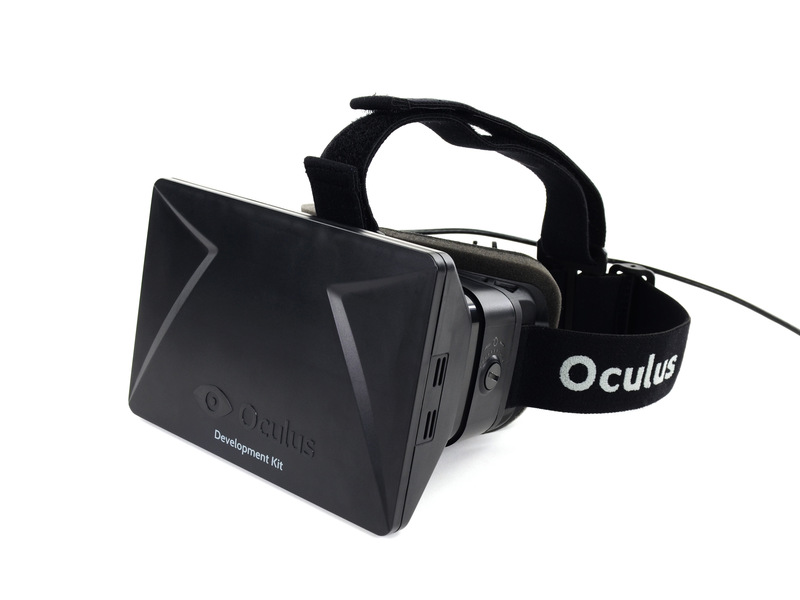
\includegraphics[width=1.0\columnwidth]{Oculus-Rift-1}
\caption{Oculus Rift}
\label{Rift}
\end{subfigure}
\begin{subfigure}{0.25\columnwidth}
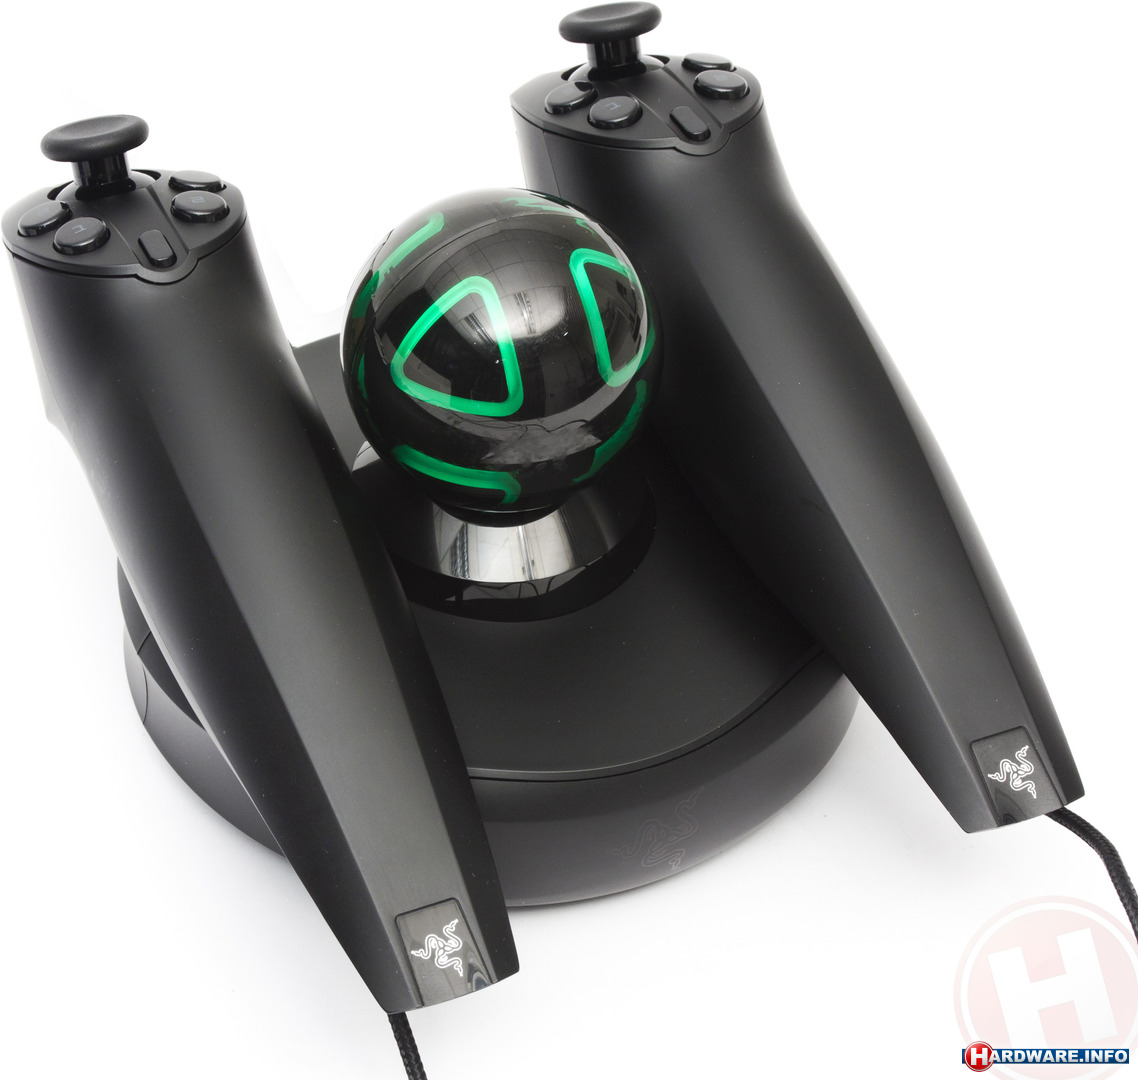
\includegraphics[width=1.0\columnwidth]{razer_hydra__portal_2}
\caption{Razer Hydra}
\label{Hydra}
\end{subfigure}
\begin{subfigure}{0.25\columnwidth}
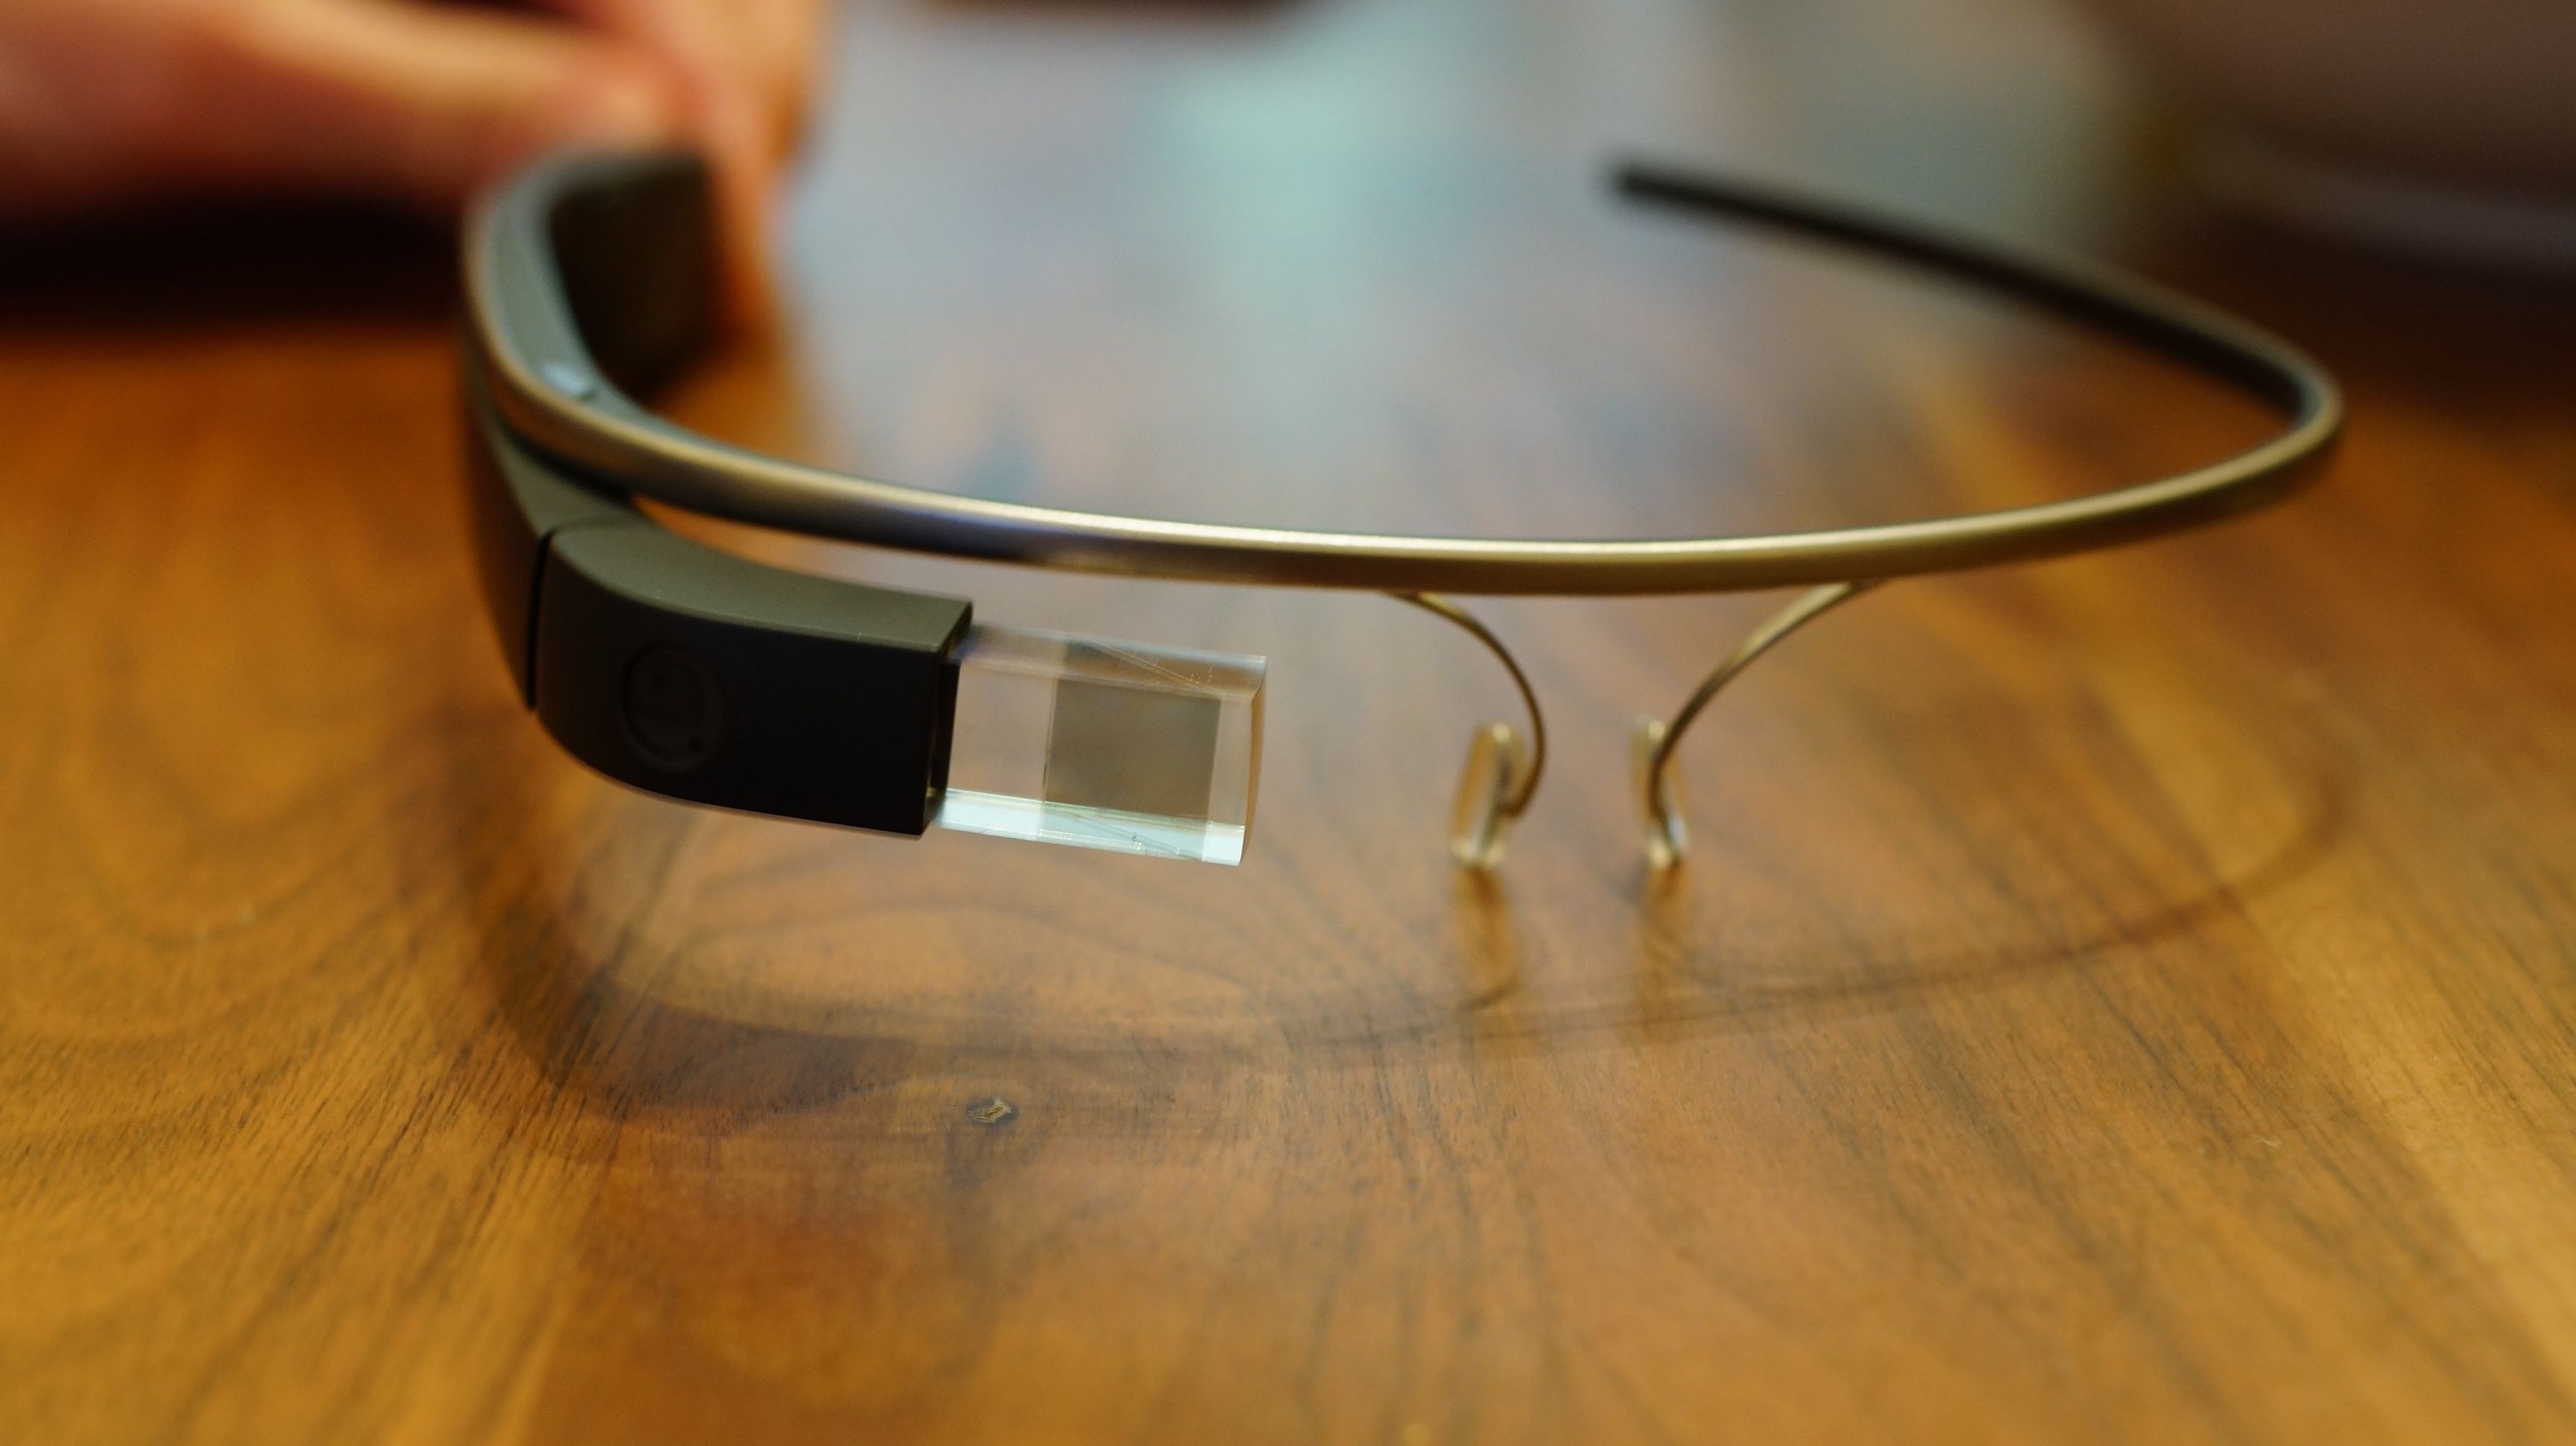
\includegraphics[width=1.0\columnwidth]{Google_Glass_Explorer_Edition}
\caption{Google Glass}
\label{Glass}
\end{subfigure}
\end{figure}

This next focus of research will involve developing a shared autonomy approach between the user, Google Glass, and the robot. The user can label objects using the Glass interface, and have that semantic mapping wirelessly sent to the robot. This semantic mapping can then be used as additional information when learning from demonstration and when giving tasks to the robot \cite{5654900}. Additionally, it can be added to the the teleoperation interface when learning and the task interface when giving commands.

For example, the robot can easily positively classify a desk, but it cannot know whose desk it is, or what the desk is used for. The user can tell Google Glass that this particular desk is his work desk, and a specific book is his class textbook. When the user later gives a task to the robot to bring the textbook to his work desk, the robot will already have this semantic information. 

\subsection{Multi-Robot Coordination}
The Robot Interactive Display Environment (RIDE) was developed by Karulf et al. to satisfy the need of a robotic control interface that allows a single user to effectively control a large number of robots \cite{hri11c}. In RIDE, operators are able to switch between direct control of a robot and supervisory control over all robots. This allows the operators as much control over the robots as the situation warrants.

RIDE was originally created to allow one user to control many robots directly, or take a supervisory role. However, the current supervisory role can be expanded to include giving high-level goals, such as bringing the user a book. Combining the abilities learned from demonstration and the semantic information obtained during object classification, we can build a new interface allowing users to give high-level goals to a group of robots.

When using RIDE to assign tasks, the user will be able to select one or more robots, and then select an object that has been given a semantic mapping. The RIDE interface will display to the user tasks that had been learned which involve interaction with this object and the selected number of robots. The selected robots will then coordinate to accomplish the task given to them by the user. These goal-based tasks will use previously-learned abilities from demonstrations. For example, we have two robots, a PR2 and Turtlebot. The PR2 is large and slow, but has limbs, while the Turltebot has no ability to interact with the environment, but is fast. Through learning by demonstration the PR2 has learned to pick up a book, and has learned to set it down, and the Turlebot has learned to move from one location to another. If the user gave these robots a task to bring a book to himself, they can coordinate these smaller tasks together to perform the larger goal. The PR2 can put the book on the Turtlebot, and the Turtlebot can deliver it.

To accomplish this, each robot will know what tasks it is capable of performing and how well it performs the task. They will will be able communicate this information with each other and coordinate. The previous example required three tasks: picking up book, setting down book, and moving. The PR2 will know it is efficient at the first two tasks, but slow at the third, whereas the Turtlebot knows it cannot perform the first two tasks, but performs the third task well. Applying this coordination allows simple robots to be able to perform much more complicated tasks when cooperating.

\section{Conclusion}
Those suffering from ALS and quadriplegia need robots in the world now, and cannot wait for full autonomy of every task. This work intends to help those suffering from severe physical disabilities by giving them the ability to teach the robot themselves, as well as easily give positive and negative feedback. By using our shared autonomy approach we separate the low-level reactivity from the higher-level reasoning, and give the higher-level reasoning task to the user. 

Additionally, this work helps reduce the cost to the end-user. By using multi-robot coordination, an expensive PR2 (\$500,000), can be replaced with a small turtlebot and a mobile arm (\$5,000 to \$20,000). This cost reduction will help bring assistive robots into the home for a greater number of people.

This work also helps further the state of the art in reinforcement learning by introducing a new Learning from Demonstration technique that uses human demonstration from non-experts. This requires robots to learn from human demonstrations, even when those demonstrations are highly suboptimal. It also furthers the field in robot coordination, allowing a robot to evaluate its own performance, and use that information to efficiently coordinate.

With these new interfaces and tools, individuals with disabilities will be able to accomplish day-to-day tasks without human assistance. The lack of a human assistant performing the task and the addition of positive experiences like teaching, doing it yourself, and being more independent gets us closer to our goal of using robots to positively help those with physical disabilities.
%User-Centered design \cite{Abras04user-centereddesign} has been shown to be helpful in these situations. The disabled individual can be considered a super user, and drive the design process  \cite{journals/ram/ChenCCGHHKKLLNPPST13}. 

%REPS can be used to weigh the quality of data points. Removes bad data points from handicap teachers.

%For example, teleoperation is rarely used with high degree of freedom humanoids, since their complex motions are typically difficult to control via joystick

%Fong, Thorpe, and Baur - Ask for help. Useful!

%User-Centric design. LfD.


\clearpage

\bibliographystyle{plain}
\bibliography{../thesis}

\appendix

\end{document}
